%!TEX root = main.tex
% Begin: INTRODUCTION %
\section{Introduction}
High school students in the Netherlands face challenges while keeping up with courses and preparing for exams.
Effective preparation is prevented because of boredom, low motivation and frustration \cite{Ford2013,Shernoff2003StudentTheory.}.
These feelings often stem from missing relevance of study material in regard to the daily life of students \cite{Shernoff2003StudentTheory.}
This is not only troublesome for passing the exams at hand but also has a negative effect on long-term motivation and lowers trust in education systems \cite{Ford2013}
It can also lead to students focusing exclusively on scoring high in exams and turning away from actual learning \cite{Fitzgerald2000TestsStudents}.
Rather than replacing traditional learning and exams as a form of assessment this paper focuses on complementing learning in a way that increases short-term motivation prior to exams and preserving long-term motivation for future education.

Games typically engage their players in intensive sessions. During such a session a player is focused on the games activities and has to learn the associated concepts in order to reach given targets \cite{Przybylski2010AEngagement.}. Utilizing this immersion has proven itself to be valuable for serious and educational games \cite{Garris2002}.
This paper describes an intelligent, serious game which engages students playing it while implicitly facilitating the topic \enquote{Human Immune System} in Biology.
It is not meant to be actively used in a teacher classroom setting. Instead it should allow students to use it as a complementing tool in conjunction with learning.
Abstract concepts can be made more approachable in the game and recognized by students. It allows for visually appealing representations of the components involved and features elements which can be easily transferred into a game. The objective of shielding the human body from harmful bacteria and viruses can be used as the main goal throughout levels. In addition to that white blood cells function as protagonists while bacteria and viruses represent the antagonists.

A constant adaption of the games difficulty will help to challenge the player and sustaining motivation. Challenging the students abilities can also improve the learning effectiveness \cite{Hamari2016}.
The game will dynamically adapt to the knowledge of the player about the immune system. It makes use of a \textit{Learner Model}\cite{Nguyen2008LearnerLearning} to approximate the player's knowledge within the system. Increasing difficulty means introducing new cells, organs, threats and effects into the gameplay. Effectively scaling up the amount of variables and interactions in play.

Given the ubiquitous presence of smartphones nowadays and the relatively young age of high school students the target platform of the game is mobile \cite{Harris2013PearsonStudents}. Being built on web technologies the game is also distributed to be executed in modern web browsers. This accommodates for students without access to a smartphone \cite{Lenhart2015TeensTeens}.
% End: INTRODUCTION %

% Begin: RELATED WORK %
\section{Related Work}
\subsection{Intelligent Educational Systems}
\textit{Intelligent educational systems} map the learner's knowledge to internal representations \cite{Ma2014}. Making use of this state allows them to dynamically adapt instructional processes to the user's progress within the subject domain. In a meta-analysis by Ma et.al \cite{Ma2014} results showed positive effects regarding learning outcomes when intelligent, educational software was used. It also supports the claim that using it as a secondary, complementary learning tool does not hinder effectiveness. Furthermore, the use of these systems is not restricted to a small group of subject domains; usage within the field of Biology has moderate, positive effect sizes \cite{Ma2014}.

According to Khenissi et al. \cite{Khenissi2015} the \textit{Learner Model} is a central component within adaptive learning environments. It is responsible for modelling \enquote{the knowledge, difficulties and misconceptions of the individual} \cite{Bull2013OpenProcesses}.

\subsection{Serious Games}
Learning and retention of knowledge can be effectively supported by \textit{Serious Games} \cite{Wouters2013}. Moreover, the analysis by Wouters et al. \cite{Wouters2013} revealed that using serious games alongside traditional learning techniques leads to better learning outcomes.

Educational games are able to improve motivation and engagement with the presented study material \cite{Khenissi2015}.

\subsection{Mobile}
In 2015 a mobile, meaningful learning system was developed to teach high school students about the, rather complex, blood circulation in the field of Biology \cite{Fan2015TheCurriculum}. The in-game material's design aims to reflect the conventional teaching material used for the control group of the study. Both learning effectiveness and exam results showed significant improvements for the group of students using the mobile game.

Mobile education has the ability to improve on traditional learning methods which do not necessarily meet the requirements of the mobile-era \cite{Sciences2015MobileScenario}. It integrates with modern, mobile lifestyle by making use of smartphone technologies. Mobile technology is a central area for research in the field of teaching and learning \cite{Ally2014WhatEducation}.

% End: RELATED WORK %

% Begin: INTERACTION %
\section{Interaction Design}
This section will focus on all aspects of the interaction between the user and the game.
A popular model in user experience by J.J. Garrett consists of five layers going from an abstract concept to a more concrete idea \cite{Garrett2000InterfaceObjectives}.
The layers, or planes, build on top of each other and form a guideline during the design process.
Starting out with the first, abstract \textit{Strategy Plane} section \ref{persona} explains the user needs according to a persona of a potential high school student. In addition to that \ref{requirements} lists the specific goals the project is set to achieve.
Moving on to the less abstract \textit{Scope Plane} section \ref{environment} determines target devices and technology forming the environment of the game.
The middle layer of the model, \textit{Structure Plane}, corresponds to section \ref{interface} which depicts the interface and the underlying paths the user may take.

\subsection{Persona} \label{persona}
Stacy is a student in her final year at a secondary school in Amsterdam. During the next months she will have to prepare for her final exams. After graduation she plans on achieving a degree in mathematics to become a teacher. Partly because of her strong interest in maths she has problems motivating herself for other subjects which she deems less relevant. Nevertheless she pushes herself to prove to her parents and peers that she is doing well. Apart from taking part in a sports team and watching TV series most of her time is spent online on social media platforms and playing casual games from time to time. Her smartphone is an integral part of her life and is also used in social settings with her friends.

Stacy could make use of a game like Wreck Sam to approach study topics with low interest from a different angle. The combination of visual elements and an interactive experience allows her to connect with the theoretical concepts from her study materials. Even in cases where she did not prepare for a lecture the game could be helpful. Playing it beforehand equips her with the minimum understanding required to follow along in school. While it does not free her of reading up on the discussed topics afterwards, it lowers the potential of frustration and loss of motivation by feeling lost.

Furthermore, engaging in the game can act as a mental pause and changing her focus on a different medium. She is also able to make use of her time on public transport or in moments of boredom requiring a useful distraction. Exchanging with her friends about game mechanics and strategies acts as a \textit{"Learning-through-teaching"}-Effect \cite{Webb2016Learning}.

Of course, Stacy might decide to play the game either during class or before going to bed. Both of these situation are not entirely ideal and countermeasures should be implemented.
Using it in school keeps her from paying attention. As it is not meant to replace traditional learning techniques this should be avoided.
Playing before sleeping and thereby repeating the content can help her to reinforce the knowledge \cite{Gais2006SleepRecall}. However, it also prevents her from actually sleeping. Moreover, the light emitted by smartphone screens consists of mostly blue light which can have a negative impact on the natural sleep cycle \cite{Tosini2016EffectsPhysiology.}.

\subsection{Requirements} \label{requirements}
This project is not meant to replace traditional learning nor is it intended as a silver bullet for exams.
Instead it should be used as a supplementary learning tool which helps a student to engage with a topic in a different way.
As most study topics can be very abstract and intangible the game should counteract this by providing a visual and interactive experience.

In order to increase intrinsic motivation and peak interest in the subject it is essential that the gameplay does not feel like a chore.
Especially superfluous repetition should be avoided as it risks further engagement and does not conform with the previous requirement.
Thus, the game needs to keep track of it's own approximation of the user's current knowledge state.

Integrating intelligent software in education allows the game to account for varying learning characteristics of students.
Therefore, it adapts to the pace of the player and can provide subtle hints for support.

To be quickly usable in any situation the game should be realized as a mobile application which does not require a constant connection to the internet.
Furthermore, it should rely on simple interactions and account for interruptions with an easy mechanism to pause and resume in cases where its used in situations like public transport.

Lastly, the system needs to take precautions against unfavourable situations which includes playing too long, in school or too late before sleeping. The goal is to provide additional support for the student to learn about the human immune system and not to create an adverse affect on school activities or daily life.

\subsection{Environment} \label{environment}
The environment specification can be split in two parts regarding the hardware and software aspects.

In terms of hardware the game will be tailored towards smartphones for mobile usage. The visual interfaced is optimised for the most popular devices\footnote{\url{http://screensiz.es/phone}, Accessed: 06-10-2017} from Apple, Google and Samsung and their respective screen resolutions and aspect ratios. Although usage in landscape mode is not restricted the recommendation is portrait orientation.

The actual software is built using web technologies to be executed by a browser. Using Apache's Cordova\footnote{\url{https://cordova.apache.org/}, Accessed: 06-10-2017} multiple distributions can be created for running in a browser or in a native context on iOS or Android phones as apps.

\subsection{Interface} \label{interface}

\subsubsection{Setup} \label{setup-interface}
When starting the game for the very first time the setup screens will be shown (Figure \ref{fig_setup}). They consist of two minimalistic steps asking for the given name and age. Each interface is composed of three sections from top to bottom: Prompt, input and navigation. These forms are designed to be easy to fill out in order to minimize intrusiveness.

The prompt section is represented by header text asking for the required input, respectively \textit{\enquote{What's your name?}} and \textit{\enquote{How old are you?}}. Input elements are centered and enlarged to draw attention. Lastly, the navigation area is made up out of a prominent button which continues to the next step and two dots below. They highlight the current active step and allow the user to go back by tapping on them.

After completing the setup the gathered information (name \& age) is saved to the \textit{User State} (Section \ref{user-state}). Future game sessions will skip the \textit{Setup} and continue directly to the \textit{Main Menu} (Section \ref{main-menu}). First time players are taken to the \textit{Tutorial} (Section \ref{tutorial}) after finishing the \textit{Setup}.

\begin{figure}[H]
  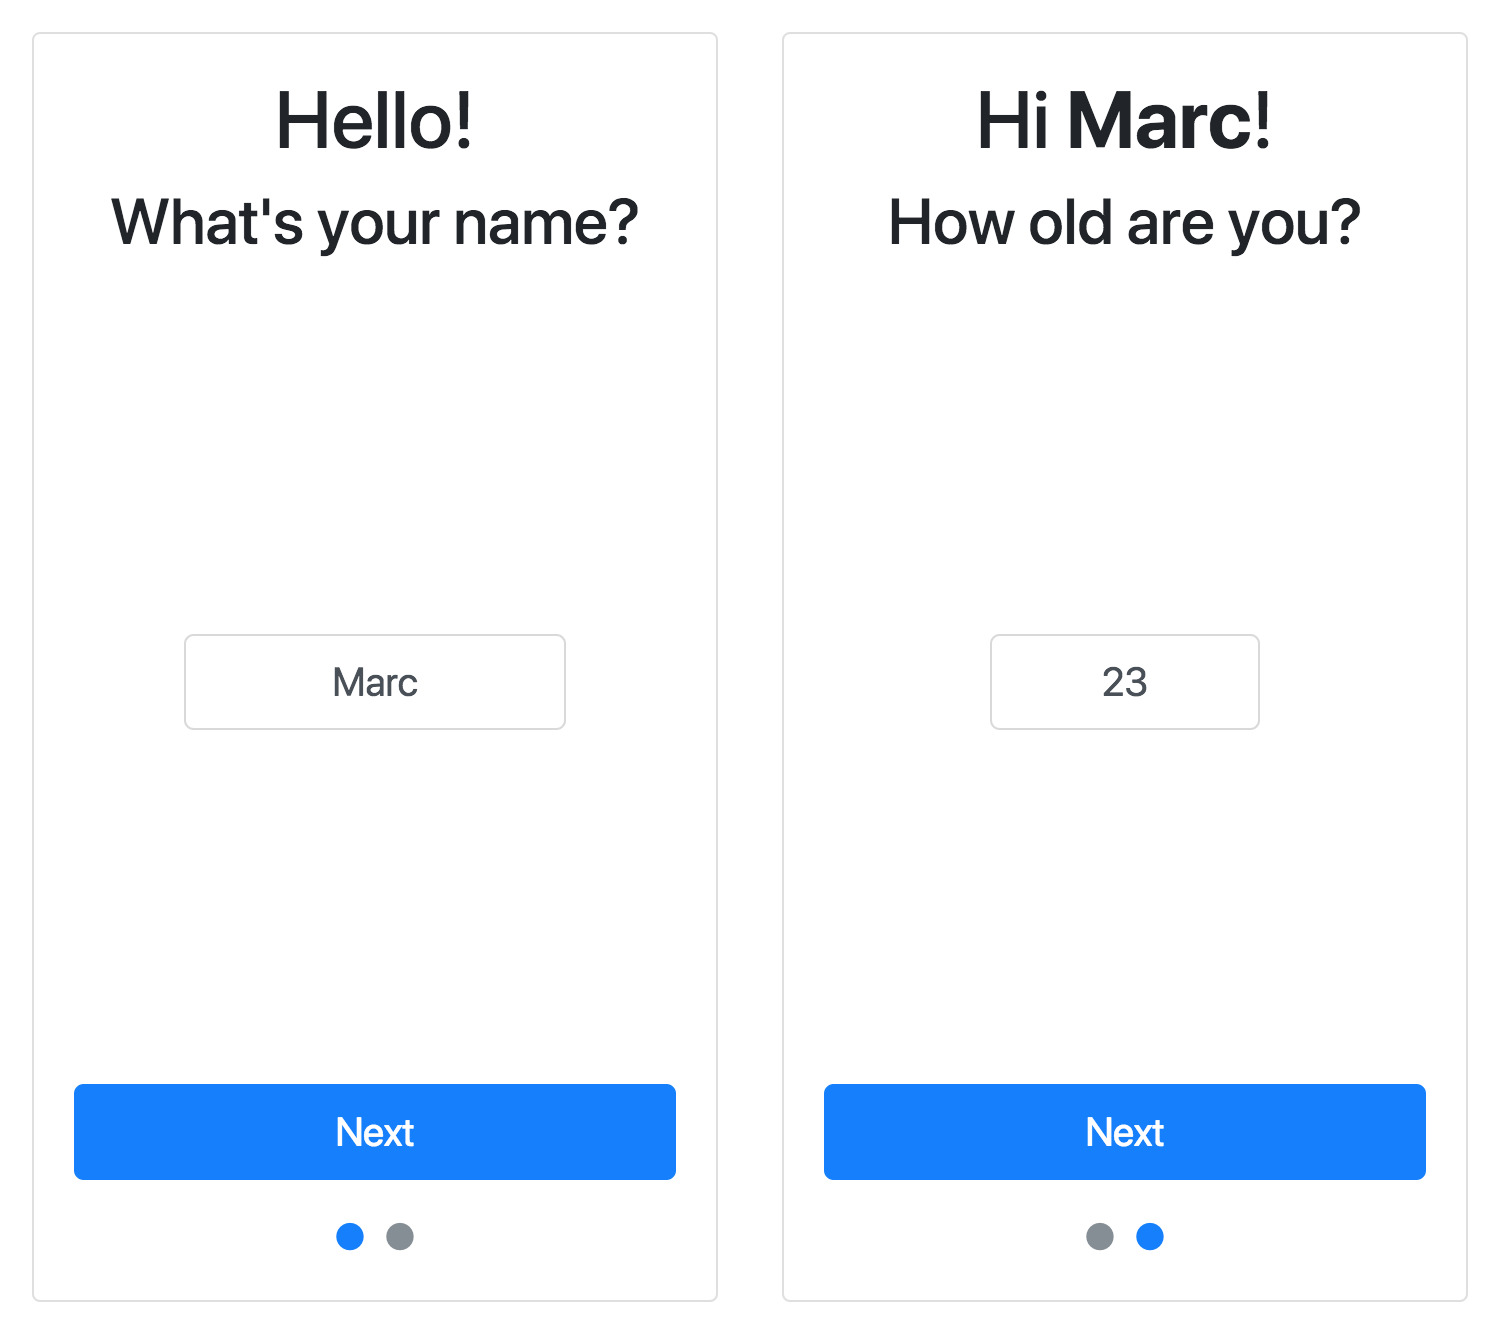
\includegraphics[width=5cm]{assets/mockup_setup_combined.jpg}
  \caption{Wireframe of setup screens}
  \centering
  \label{fig_setup}
\end{figure}

\subsubsection{Tutorial} \label{tutorial}
Coming from the \textit{Setup} a new player automatically starts with the \textit{Tutorial} afterwards. This is intended to progressively introduce core game mechanics and elements to the player. While the following paragraphs proposes a text-centric approach for giving explanations it is possible to enhance this interaction by adding audio voice overs. Providing audio is explored in \textit{Discussion (Section \ref{discussion})} and \textit{Future Work (Section \ref{future-work})}.

Harmful bacteria has infected the body through a wound. At the very beginning the user has a passive role and waits for the tutorial to present new content (Figure \ref{fig_tutorial_wireframes}, WF1).
The amount of bacteria is visible next to the cell and starts growing exponentially.

When a certain threshold is hit a blocking alert introduces \textit{Macrophages (m$\varphi$)} as a defense mechanism (Figure \ref{fig_tutorial_wireframes}, WF2). It highlights the use of this type of cells, features what they look like and explains the required action by the player to make use of them. As long as a blocking alert is visible the game activity is paused. The alert can be dismissed by tapping the \textit{'I got it'}-button.

In case the user is interested in reading more about the presented cell a secondary \textit{More information}-button is present (Figure \ref{fig_prototype_alert}). Invoking this button opens the corresponding \textit{Wikipedia}\footnote{\url{https://www.wikipedia.org/}, Accessed: 24-10-2017} page using an in-app browser\footnote{\url{https://github.com/apache/cordova-plugin-inappbrowser}, Accessed: 24-10-2017} (Please note: The \hyperref[prototype]{Prototype} implements external links for simplicity reasons). Using the in-app browser avoids actually leaving the application; the user is able to simply close the overlay when finished. Future iterations of the game could provide self-curated content instead of relying on \textit{Wikipedia} or cooperate with schools.

\begin{figure}
  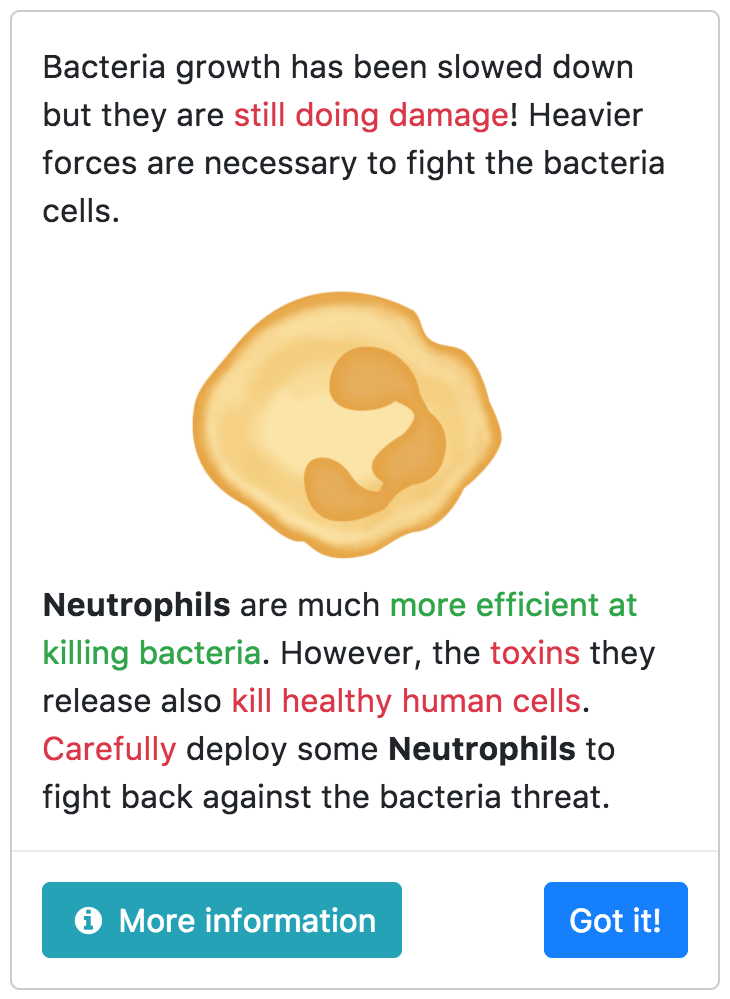
\includegraphics[width=5cm]{assets/prototype_modal.png}
  \caption{\textit{Neutrophil} alert during the tutorial}
  \centering
  \label{fig_prototype_alert}
\end{figure}

After dismissing the first alert the \textit{Macrophages} are added to the white area at the bottom of the screen which represents bone marrow (Figure \ref{fig_tutorial_wireframes}, WF3). This acts as a repository of defensive cells the player can activate by dragging them to the upper tissue-area. The game monitors whether the user actually uses the newly introduced action. If it observes an ongoing inactivity a transparent animation demonstrates the expected drag and drop motion.

Once active \textit{Macrophages} are in the tissue the bacteria growth rate is reduced (Figure \ref{fig_tutorial_wireframes}, WF4). The \textit{Macrophages} consume bacteria cells by eating them which is visualized by an animation. Adding more defensive cells to the tissue will further decrease bacteria growth but another alert informs the player that the bone marrow is unable to produce new white blood cells without stem cells (Figure \ref{fig_tutorial_wireframes}, WF4.2). After acknowledging this alert the player faces a growing amount of bacteria without countermeasures for a short period of time.

Similar to the \textit{Macrophages} introduction a new alert explains \textit{Neutrophils (neu)} as an additional, more effective white blood cell (Figure \ref{fig_tutorial_wireframes}, WF5). They can be activated by tapping \textit{Macrophages} in the tissue which opens a radial menu\footnote{\url{https://en.wikipedia.org/wiki/Pie_menu}, Accessed: 06-10-2017} around the cell (Figure \ref{fig_tutorial_wireframes}, WF6). As with every new action the game measures inactivity to provide a supporting animation to the player.

Having \textit{Neutrophil} cells in the tissue drastically reduces bacteria growth. After a few seconds an alert points out that, although \textit{Neutrophils} are effective against bacteria, they also exert negative side effects on the body by releasing toxins (Figure \ref{fig_tutorial_wireframes}, WF8). This negative property mimics actual \textit{Neutrophils} in the human body. Again, the player is able to read more about this cell using the \textit{More information}-button (Figure \ref{fig_prototype_alert}). Animating the release of toxins inside the tissue area helps to visualize this ongoing process (See also Section \ref{future-work}).

One of two conditions leads to \textit{Tutorial} completion. If (1) the amount of bacteria cells drops to zero or (2) the health bar (given in percent) is depleted to zero (Figure \ref{fig_prototype_loosewin}). Eradicating bacteria cells is achieved by deploying \textit{Macrophages} and a low number of \textit{Neutrophils}; otherwise they would hurt the body too much before reaching their goal. Health is influenced by the amount of bacteria and \textit{Neutrophil} cells active in the tissue and represented as a horizontal percentage bar at the top of the screen (Figure \ref{fig_prototype_loosewin}).

\begin{figure}
  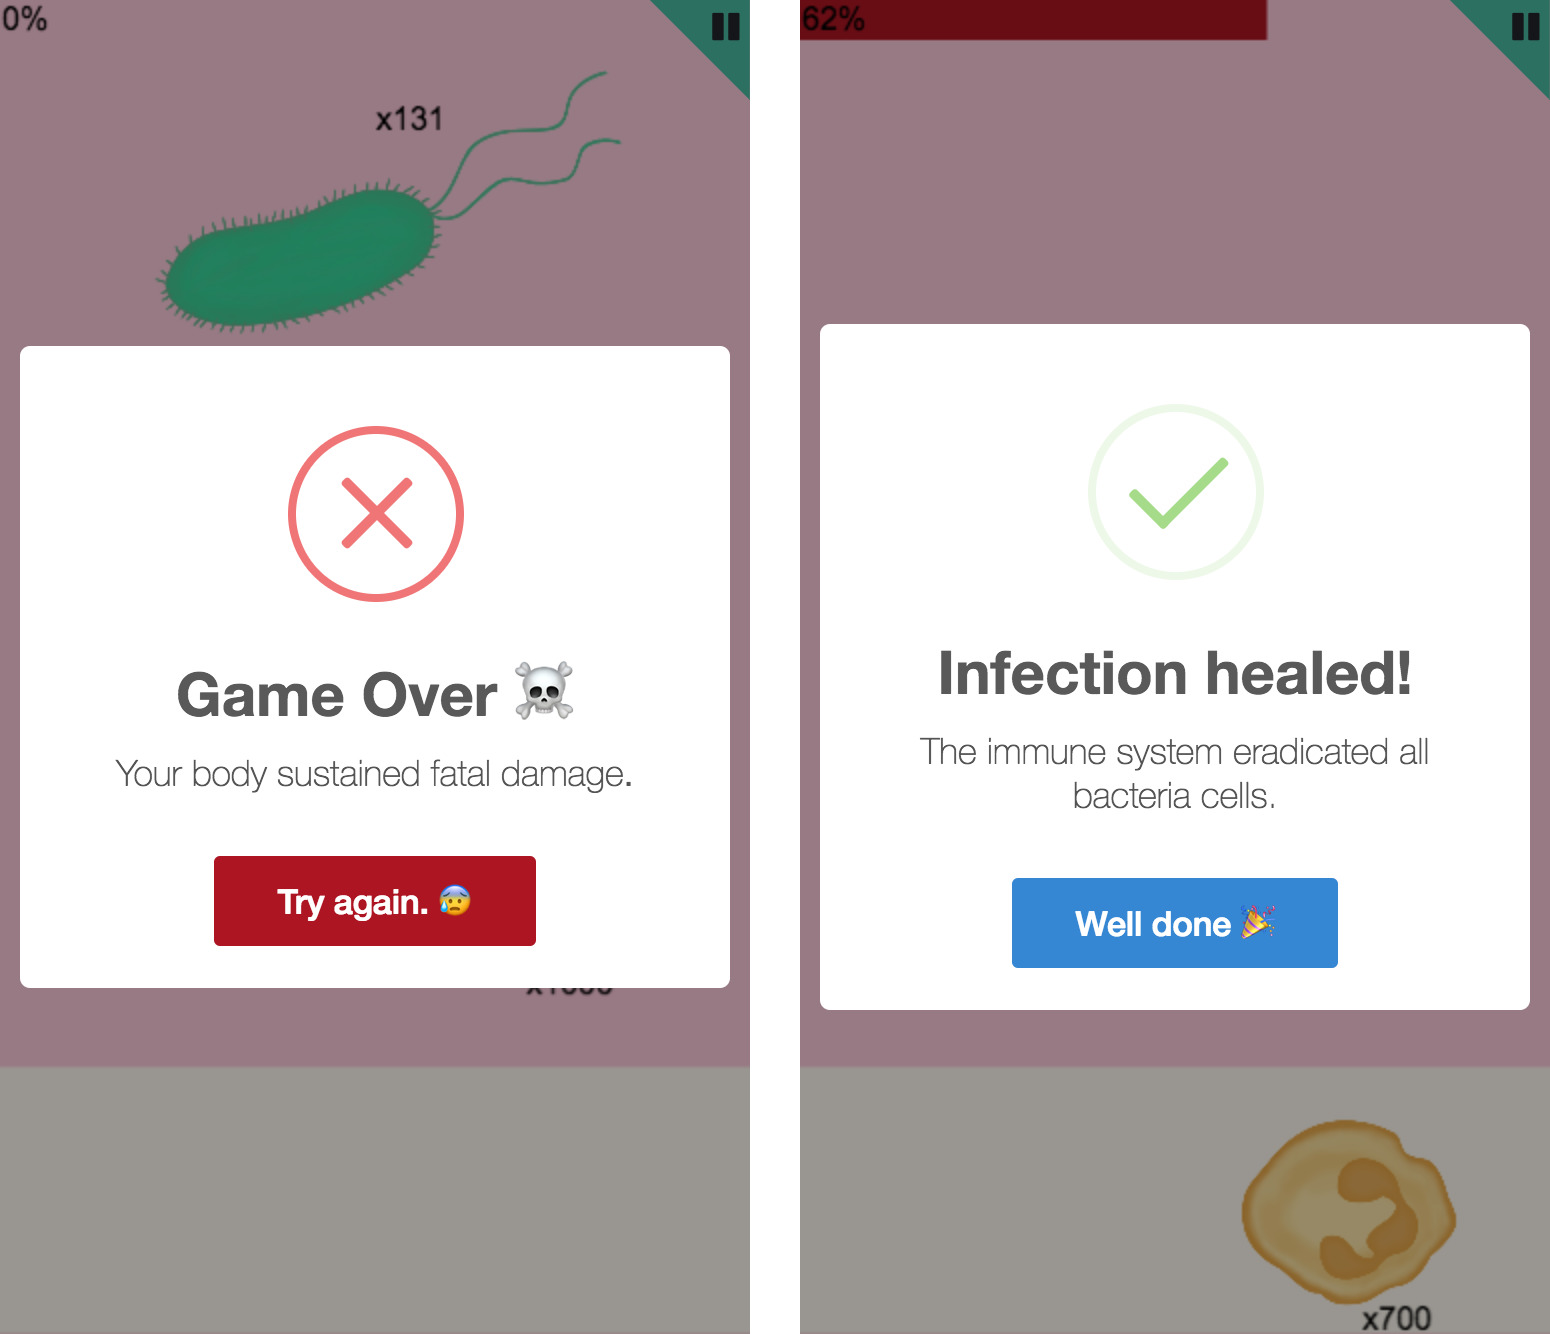
\includegraphics[width=5cm]{assets/prototype_loosewin.jpg}
  \caption{Tutorial game over and win alert}
  \centering
  \label{fig_prototype_loosewin}
\end{figure}

Completing the \textit{Tutorial}, either successful or unsuccessful, will forward the player to the \textit{Main Menu} (Section \ref{main-menu}). Furthermore, the \textit{User State} (Section \ref{user-state}) keeps track of the completed \textit{Tutorial} as it will only be started automatically once. In case of an unsuccessful attempt or the player wanting to replay the \textit{Tutorial} it can be started again from the \textit{Main Menu}.

\subsubsection{Main Menu} \label{main-menu}
The main menu screen acts as the central hub for navigation (Figure \ref{fig_mainmenu}).
The game will return to this screen after:

\begin{itemize}
	\item Showing the splash screen when starting the game
    \item Finishing the tutorial (Section \ref{tutorial})
    \item Completing or canceling a regular level
    \item Returning from settings
    \item Watching the credits
\end{itemize}

\begin{figure}
  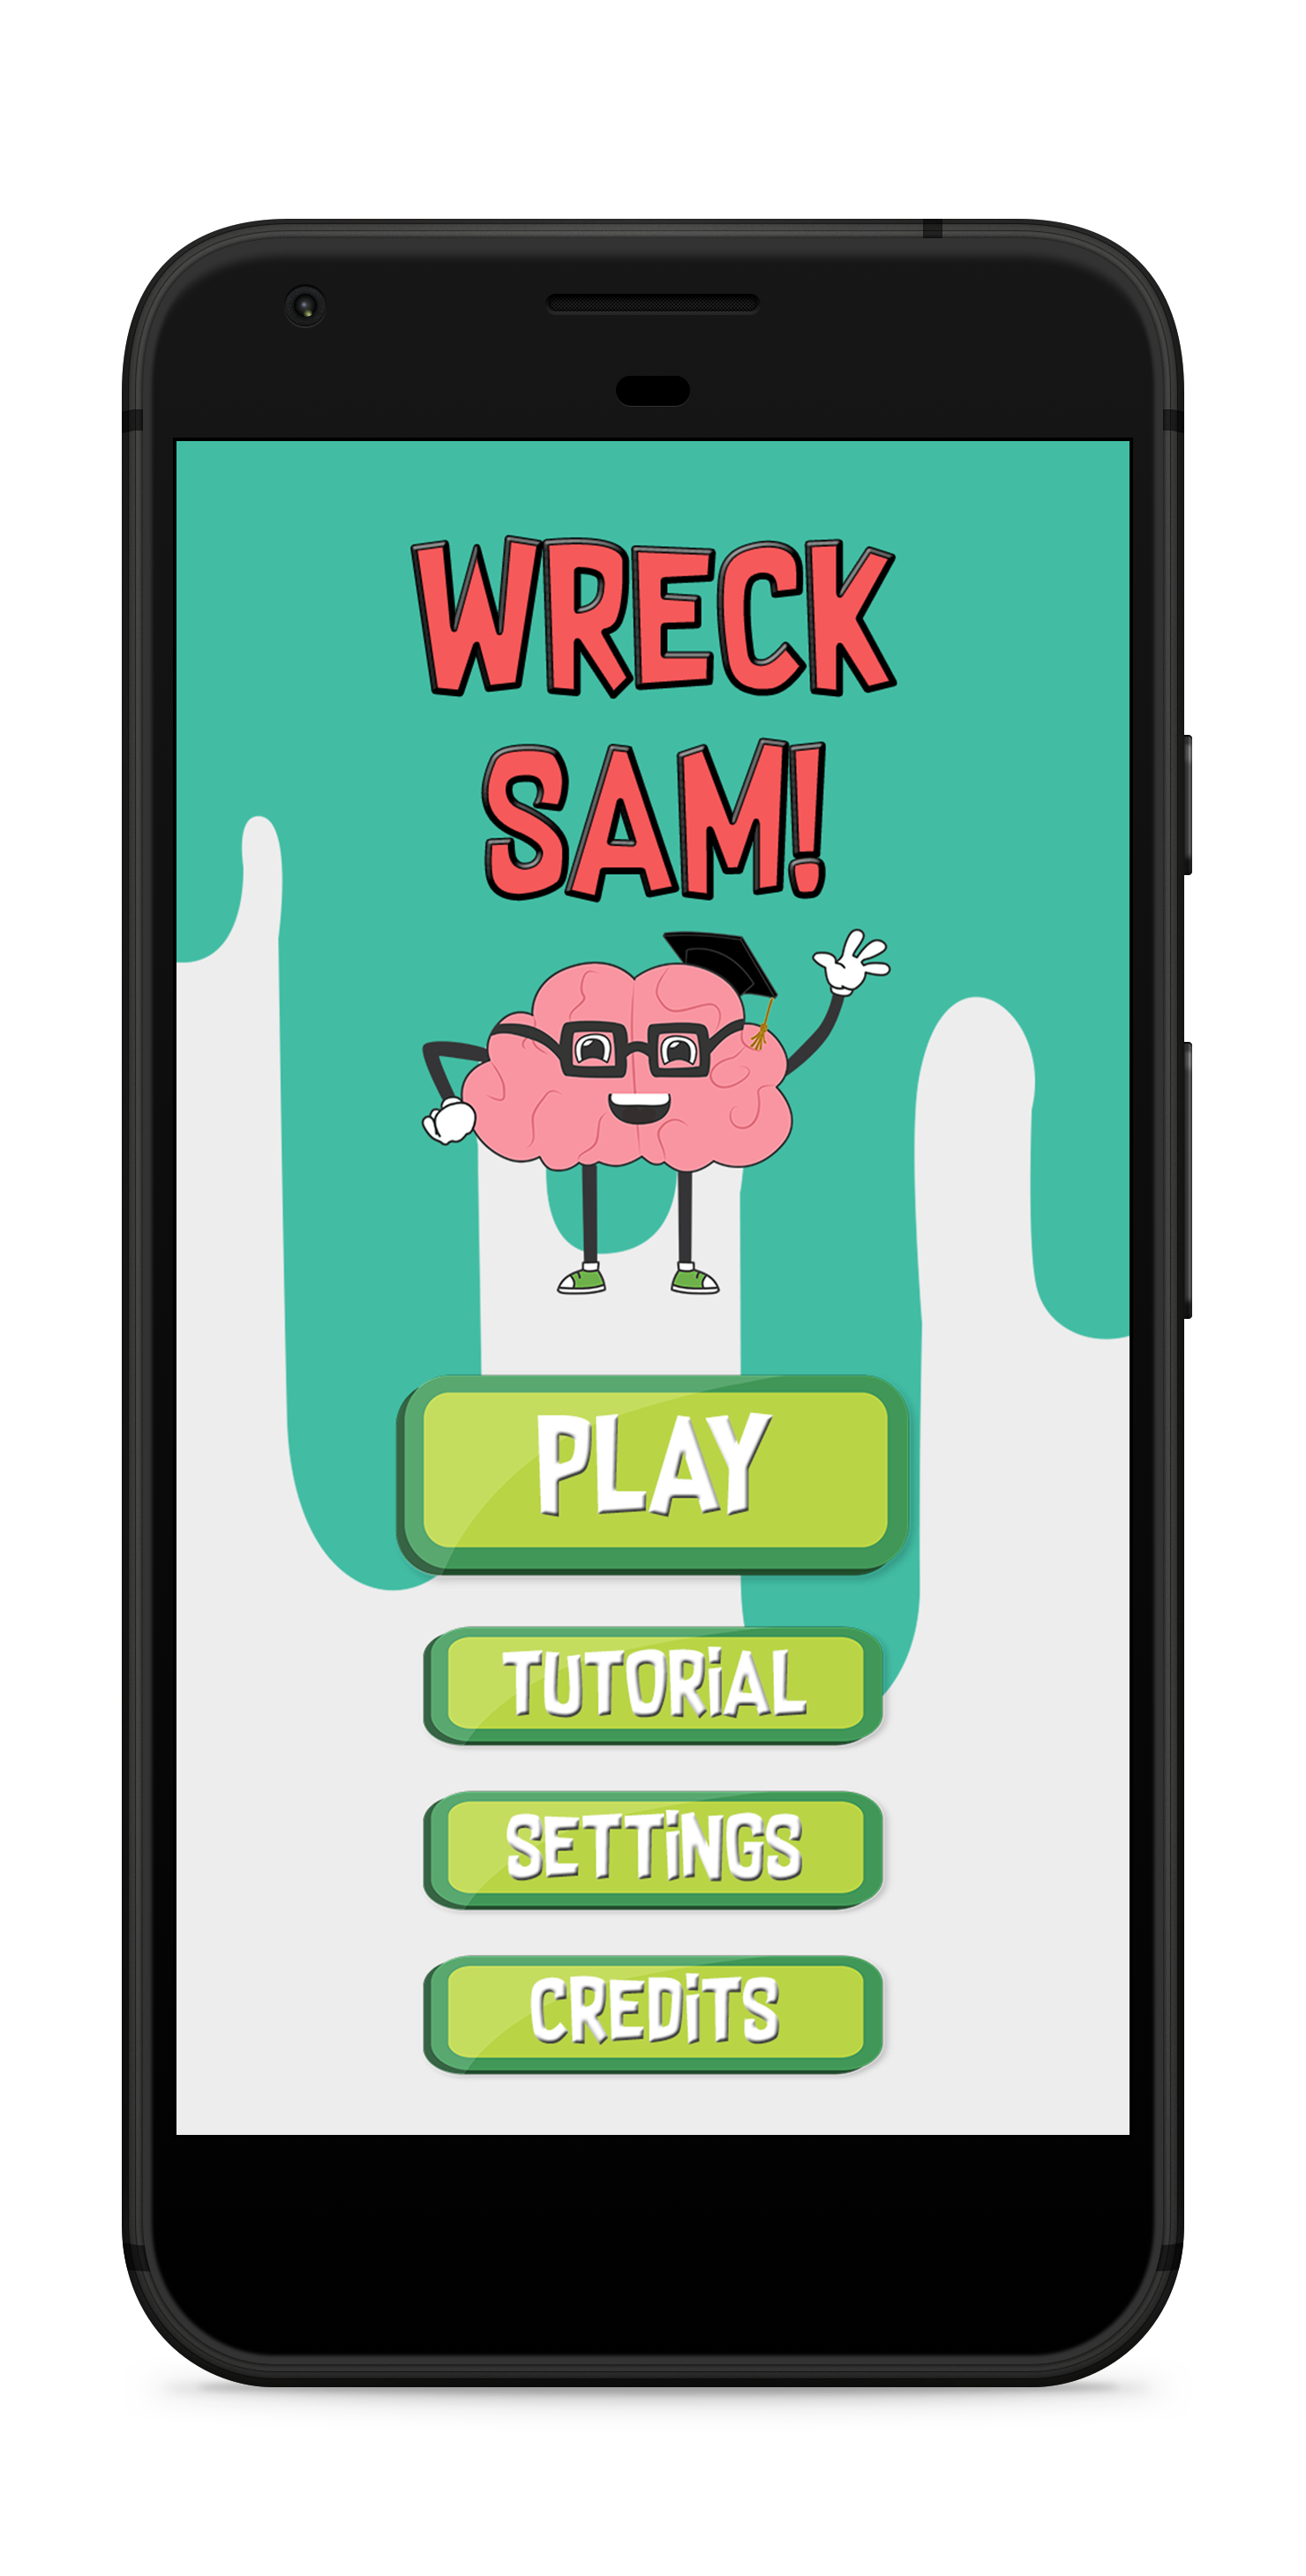
\includegraphics[width=5cm]{assets/wireframe_mainmenu.png}
  \caption{Wireframe of the game's main menu}
  \centering
  \label{fig_mainmenu}
\end{figure}

It features four prominent buttons to: Start a regular level, replay the tutorial, access settings or watch the credits. Tapping \enquote{Play} will open the body overview highlighting at which location inside the body the next level will take place (Figure \ref{fig_body}, Section \ref{gameplay}). Playing the \textit{Tutorial} (Section \ref{tutorial}) is mandatory and happens automatically when the game is started for the first time. Therefore, the player will not reach the main menu before finishing the \textit{Tutorial} once.

\subsubsection{Gameplay} \label{gameplay}
Once the user hit \enquote{Play} in the \textit{Main Menu} (Section \ref{main-menu}) the body overview will be shown (Figure \ref{fig_body}). It serves two purposes: (1) Highlighting at which location the next level will take place inside the body and (2) listing which topics from the human immune system will be included. The relevant topics are provided by the \textit{Knowledge State} (Section \ref{knowledge-state}). They are selected from an overall catalog of \textbf{23} topics:

\begin{itemize}
  \item Macrophage (See also Tutorial \ref{tutorial})
  \item Neutrophil (See also Tutorial \ref{tutorial})
  \item Natural Killer Cell
  \item Complement
  \item Mast Cell
  \item Monocyte
  \item Follicular Dendritic Cell
  \item Dendritic Cell
  \item Memory Helper T Cell
  \item Basophil
  \item Eosinophil
  \item Virgin Helper T Cell
  \item Helper T Cell
  \item Memory Helper T Stem Cell
  \item Virgin Killer T Cell
  \item Antibodies
  \item Killer T Cell
  \item Memory Killer T Cell
  \item Virgin B Cell
  \item B Cell
  \item Memory B Cell
  \item Memory B Stem Cell
  \item Memory Killer T Stem Cell
\end{itemize}

Rather than presenting the player with a classic selection of levels the body overview previews relevant elements before starting the level. The gameplay itself is similar to the \textit{Tutorial} in the sense of two mechanics. First, health is a reoccurring element in all levels. It starts out at \textbf{100\%} and must be greater than \textbf{0\%} prior to finishing a level. Secondly, the player is required to fulfill the main objective of deflecting an attack on the body e.g. killing bacteria cells, healing an infection, freeing the body of a virus, curing diseases, fighting rogue cell mutations.

\begin{figure}
  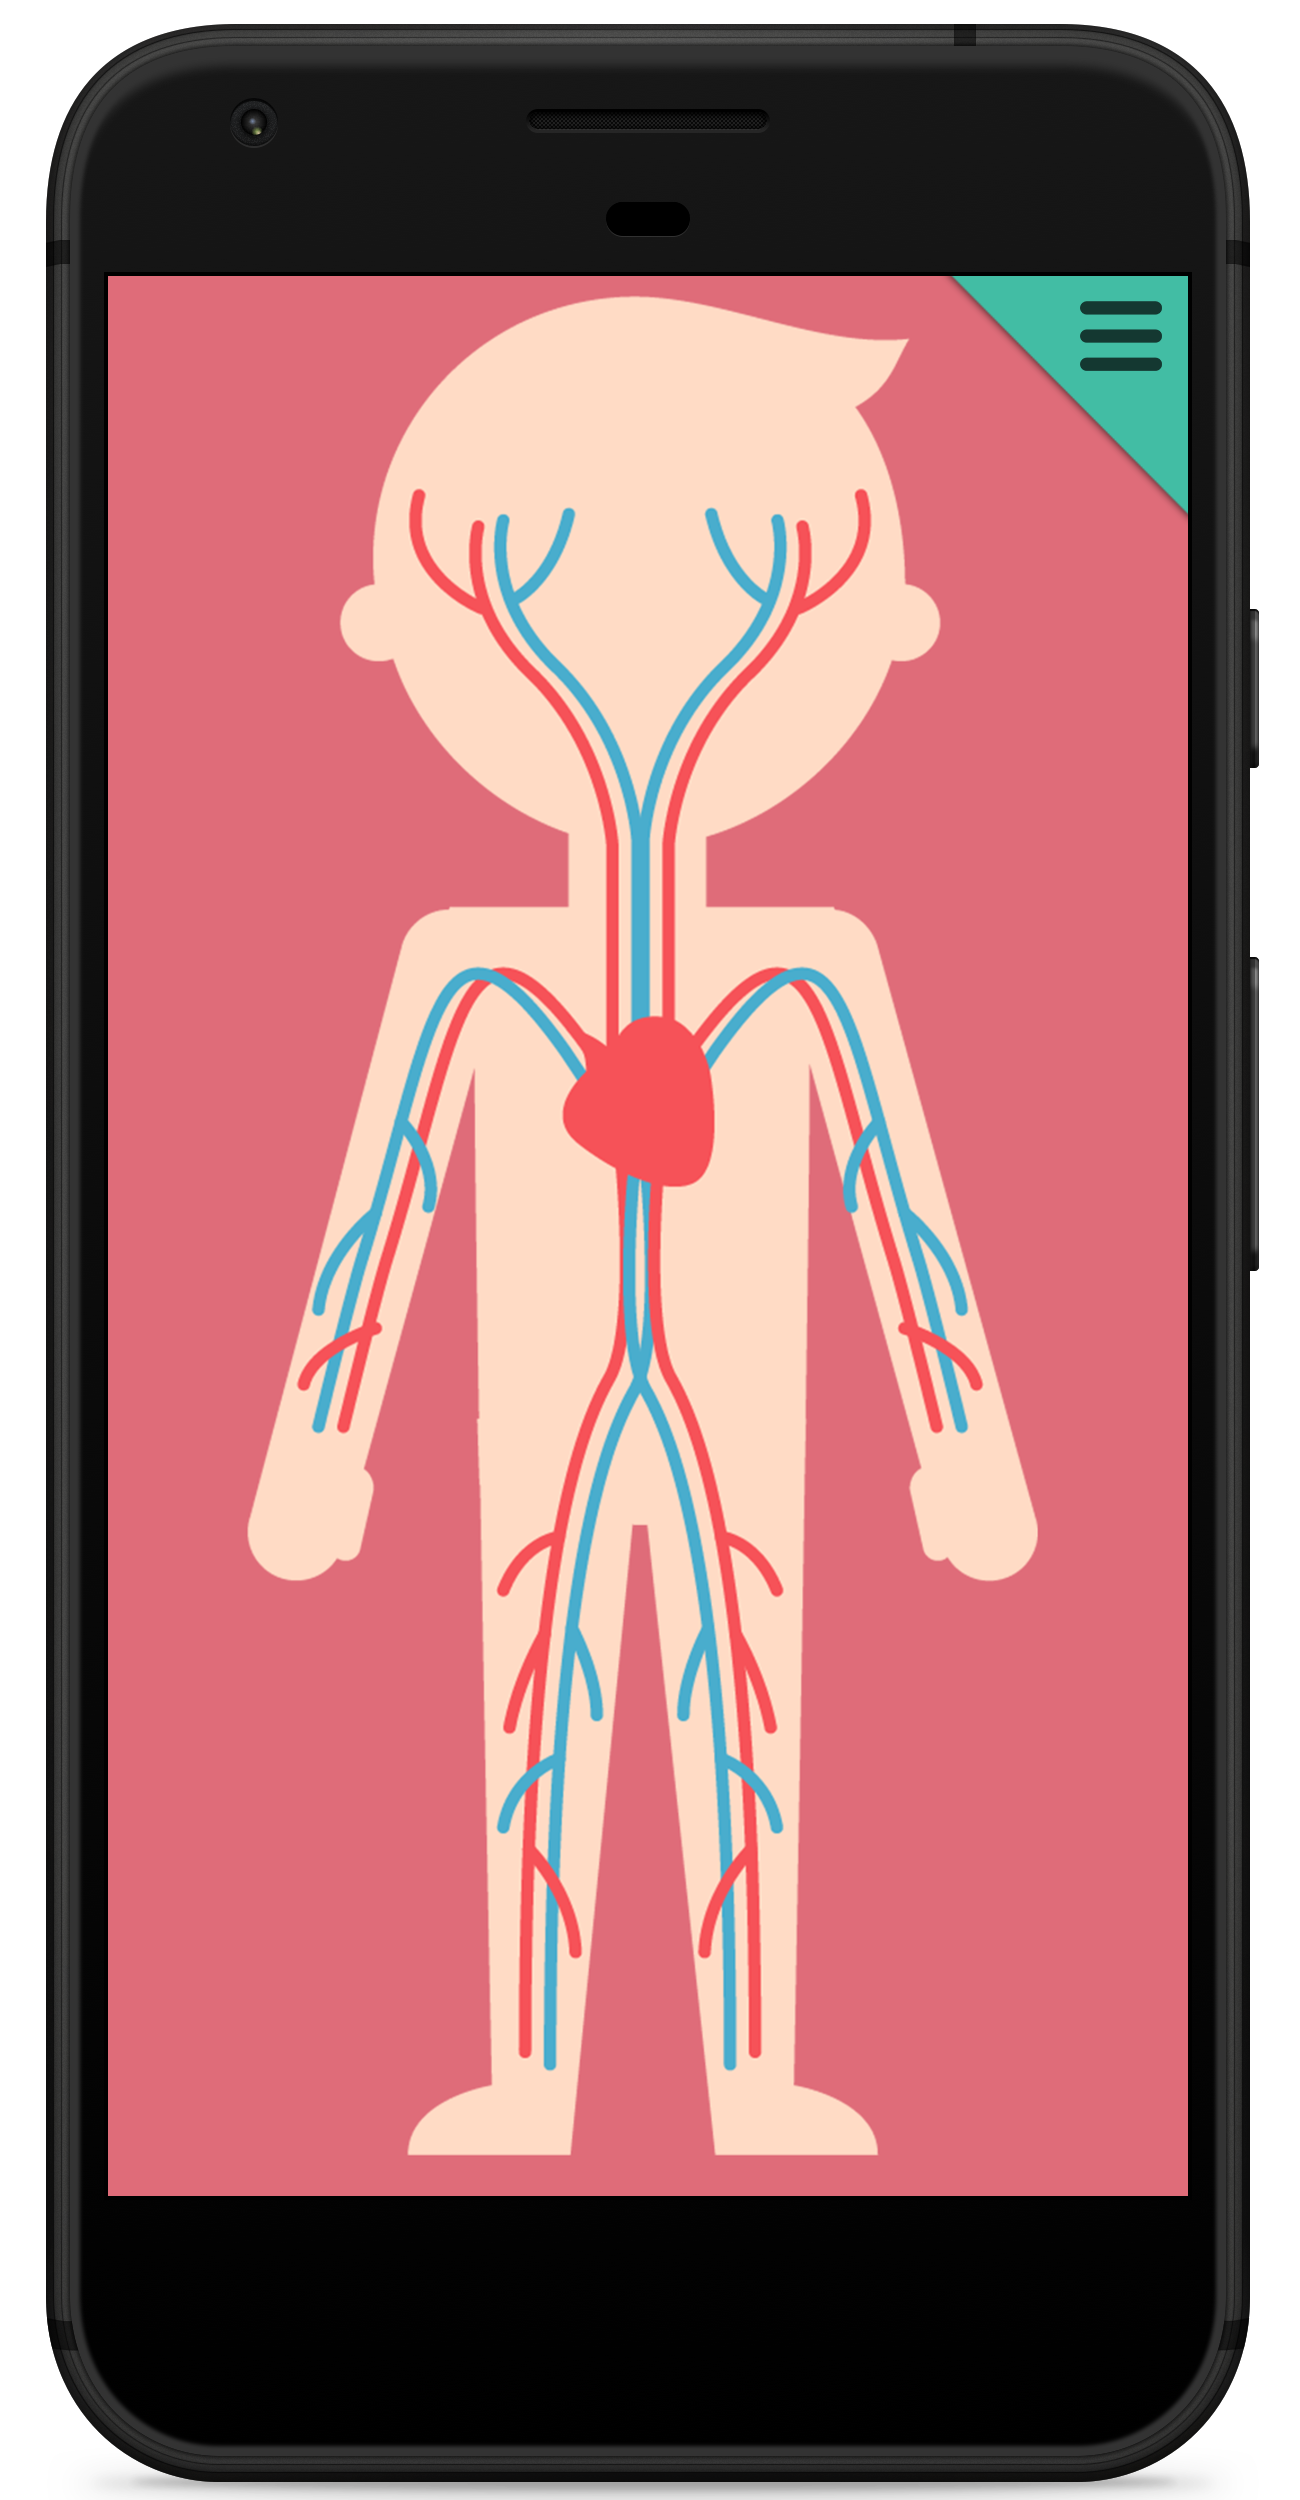
\includegraphics[width=5cm]{assets/wireframe_body.png}
  \caption{Wireframe of the body overview}
  \centering
  \label{fig_body}
\end{figure}

% Begin: Full page Interaction Design wireframes
\newpage

\begin{figure*}
  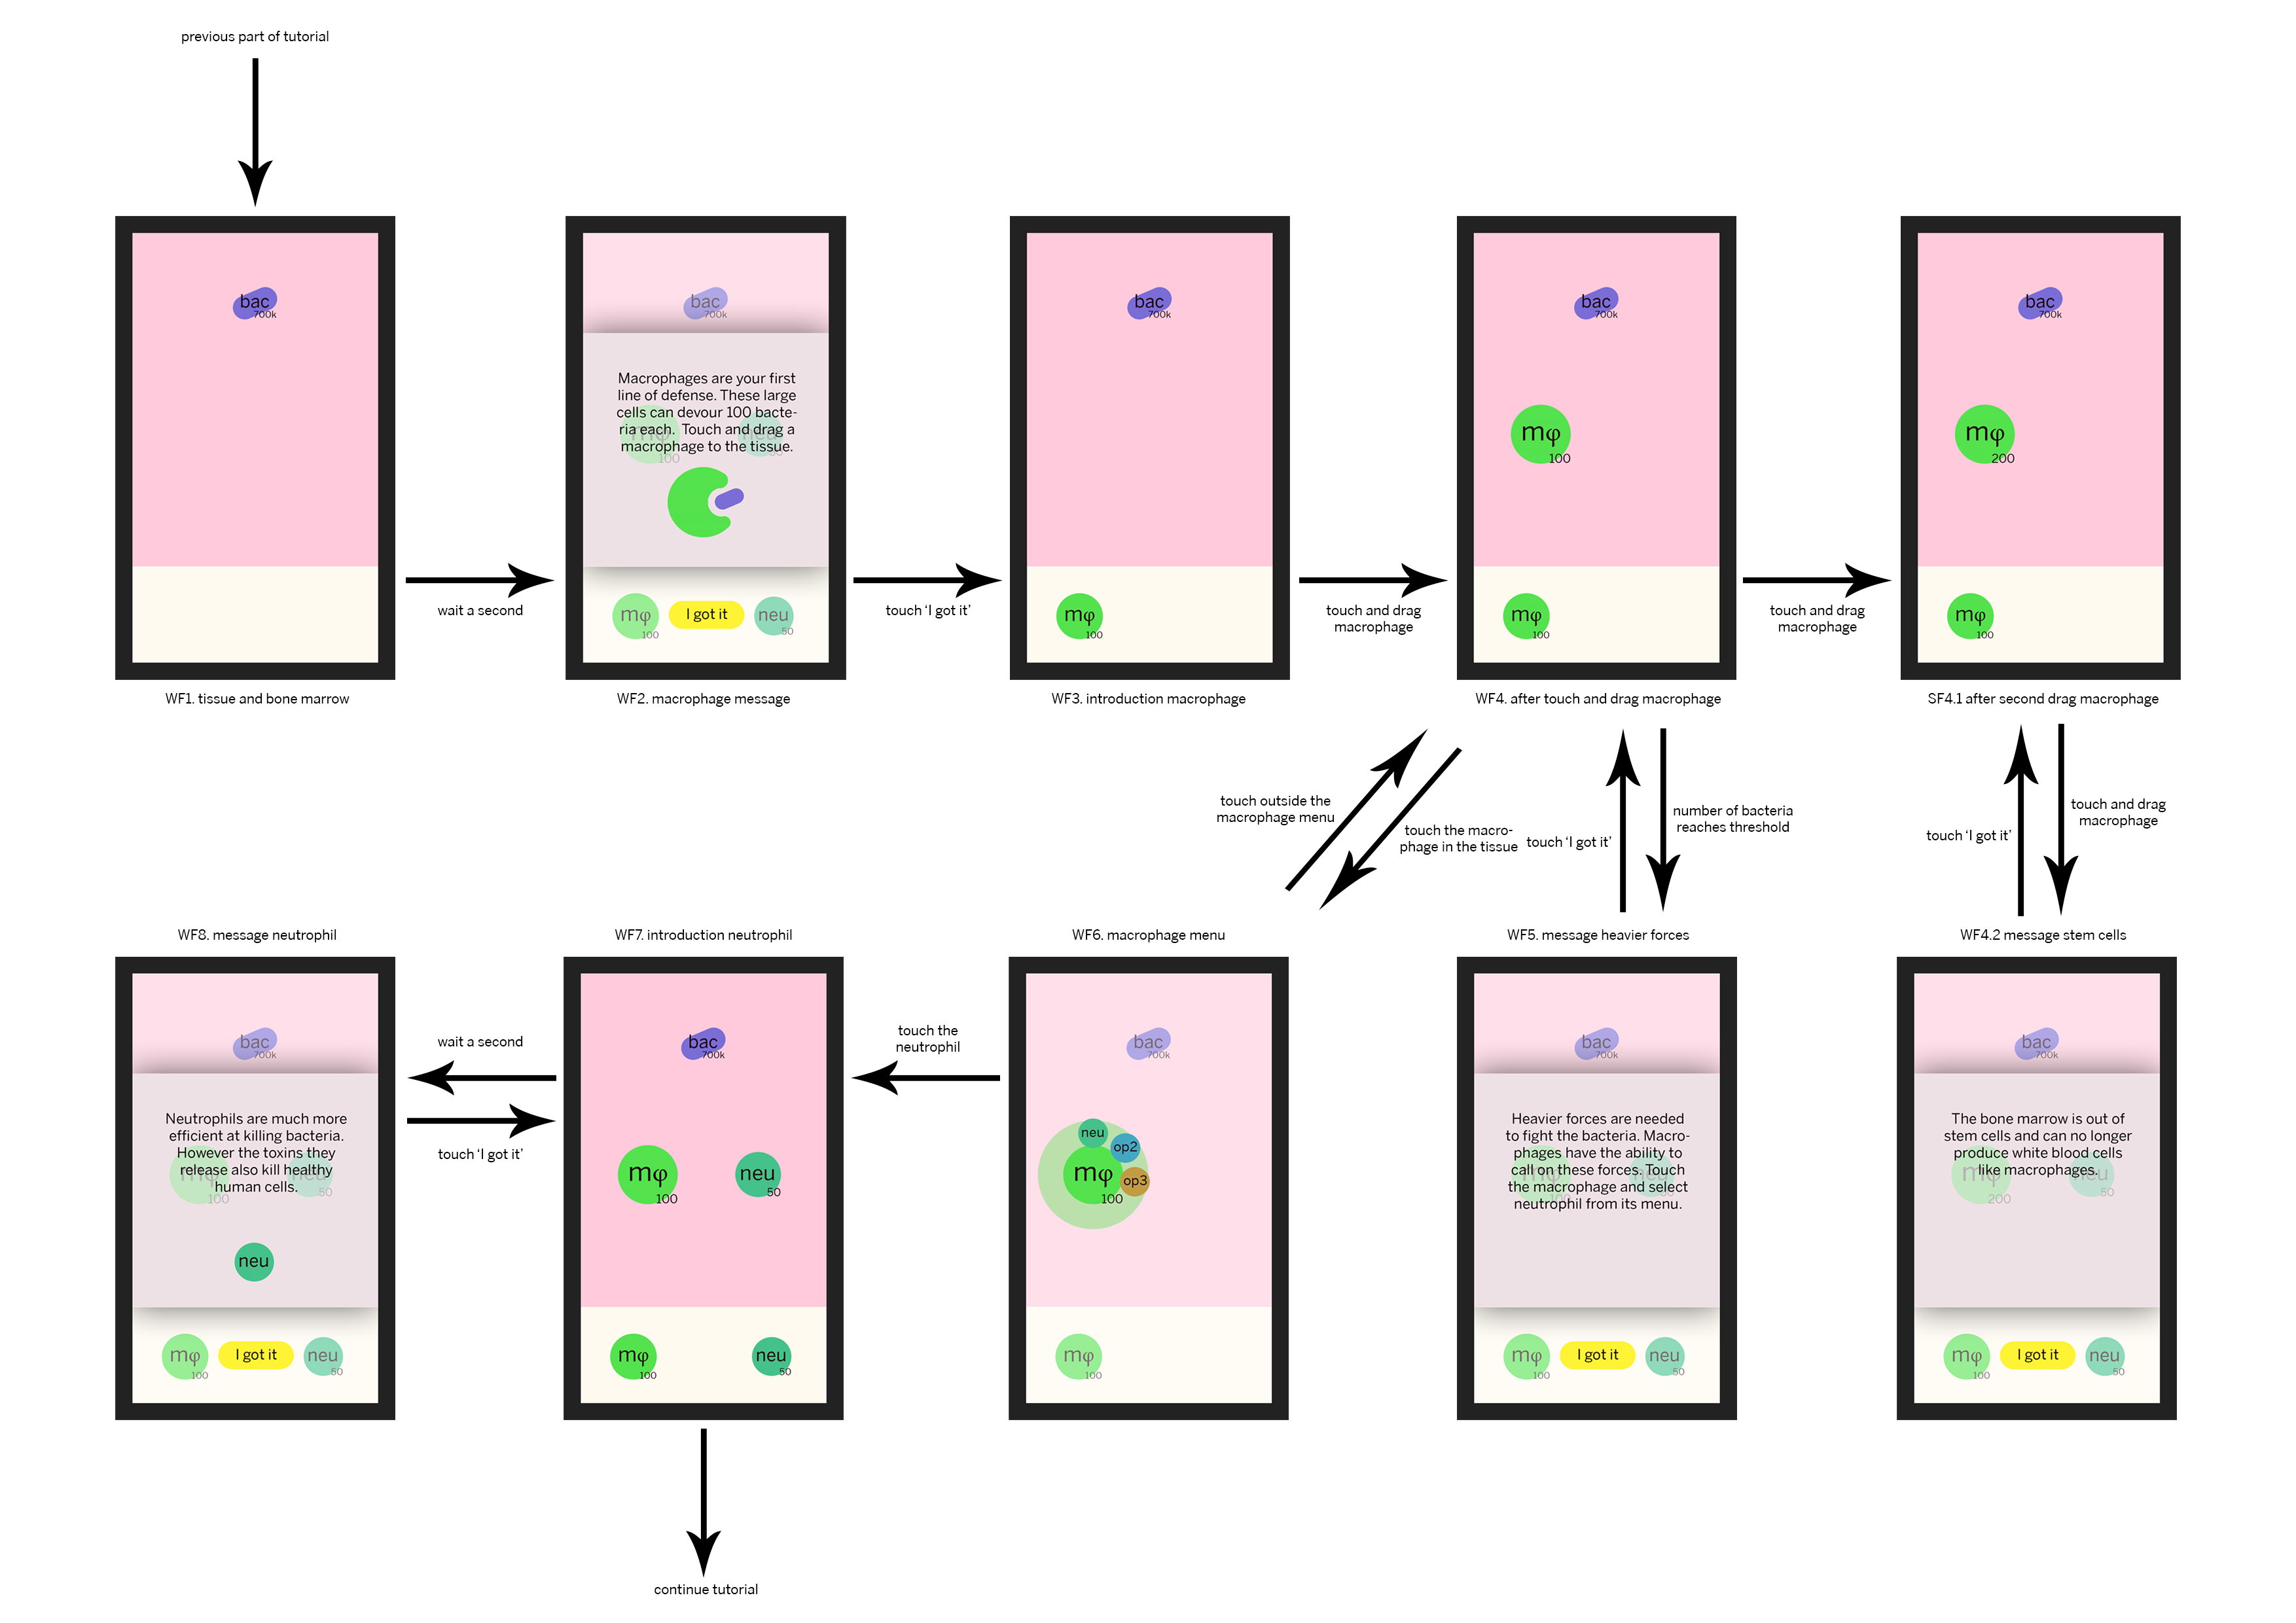
\includegraphics[width=21cm,angle=90,keepaspectratio]{assets/combinedwireframes.jpg}
  \caption{Wireframes of the tutorial flow}
  \label{fig_tutorial_wireframes}
\end{figure*}

\clearpage
% End: Full page Interaction Design wireframes
% End: INTERACTION

% Begin: SYSTEM DESCRIPTION %
\section{System Description}

\subsection{Initial Setup} \label{initial-setup}
In order to be able to play the game the user needs a smartphone. There is no strict requirement on hardware but the device should still be eligible for the support lifecycle by its manufacturer. The game itself is built upon web technologies which means virtually every device with a browser is technically capable to run the software. Being able to run the game on all devices with a browser is an advantage for students without access to a smartphone. Native apps are only provided for the operating systems \textit{iOS (Apple)}\footnote{\url{https://www.apple.com/lae/ios/ios-11/}, Accessed: 06-10-2017} and \textit{Android (Google)}\footnote{\url{https://www.android.com/}, Accessed: 06-10-2017}. This is because of the strong market share of both operating systems combined. According to a report by Gartner in 2016 the total share was 98.5\% of all smartphone sales \cite{Goasduff2017Gartner2016}. The minimum supported versions for iOS and Android are imposed by Cordova. At the time of writing the support tables for iOS\footnote{\url{https://cordova.apache.org/docs/en/latest/guide/platforms/ios/}, Accessed: 24-10-2017} and Android\footnote{\url{https://cordova.apache.org/docs/en/latest/guide/platforms/android/}, Accessed: 24-10-2017} correspond to Cordova version 7 which translates to a minimum of iOS 8 and Android 4.1. 

Although the game does not rely on a constant internet connection to be playable it is necessary to retrieve the assets for installation. The barrier of entry should be kept as low as possible, therefore two options for installation are possible.

First, the user can open a web browser and head to the official website at \textit{\url{https://marc1404.github.io/WreckSam/}}\footnote{\url{https://marc1404.github.io/WreckSam/}, Accessed: 06-10-2017}. All browsers are supported but given that something different than Google Chrome is used an advice will recommend this browser for optimal performance. As soon as the browser finished downloading and parsing the resources the game begins to run inside the browser. In a background process utilizing Service Workers\footnote{\url{https://developer.mozilla.org/en-US/docs/Web/API/Service_Worker_API}, Accessed: 23-10-2017} all assets are cached for future visits. Choosing this option the user does not need to install anything manually on the device, merely a visit to the games website suffices to start and cache the game in the background.

Secondly, the game can be installed as a native app. Distribution is handled via Apple's App Store\footnote{\url{https://www.apple.com/lae/ios/app-store/}, Accessed: 06-10-2017} for iOS and Google's Play Store\footnote{\url{https://play.google.com/store}, Accessed: 06-10-2017} for Android. This method requires a bit more effort on the user's behalf in terms of locating the app in the store and taking the necessary steps for download and installation. Yet it provides convenience in the long run. It allows to start the game directly from the smartphone's homescreen and creates a more immersive feeling due to the removal of any browser framing. Furthermore, the native environment can make more efficient use of hardware acceleration.

The decision to provide both a web version and native apps is rooted in technical as well as accessibility reasons. First and foremost, distributing the application for browsers is inherently simple when using Cordova as the underyling framework. It only involves adding the \textit{browser as a target platform}\footnote{\url{https://github.com/apache/cordova-browser}, Accessed: 24-10-2017} next to iOS and Android. In addition to that a broader crowd of potential users can be reached by including users without access to a smartphone.

\subsection{Startup} \label{startup}
After installing and running the game the startup phase is entered. If it is the first time usage the user will be prompted with two minimalistic setup screens (Section \ref{setup-interface}). The gathered information (name \& age) is stored in the \textit{User State} (Section \ref{user-state}). As soon as the user completes the setup the \textit{User State} is persisted to the web context's \textit{Local Storage}\footnote{\url{https://developer.mozilla.org/en-US/docs/Web/API/Window/localStorage}, Accessed: 24-10-2017} and send to the game server using a JavaScript \textit{XMLHttpRequest}\footnote{\url{https://developer.mozilla.org/en-US/docs/Web/API/XMLHttpRequest}, Accessed: 24-10-2017} (See also Figure \ref{fig_system_architecture}). An initial implementation for this process is available in the Prototype's GitHub Repository\footnote{\url{https://github.com/marc1404/WreckSam/blob/master/src/states/userStateService.js}, Accessed: 24-10-2017}.

During startup the system uses the current date and time to check for one of two situations:
\begin{itemize}
	\item In school usage
    \item Late playing
\end{itemize}
If it is a weekday and the time roughly corresponds to the time window of high school an alert reminds the user to pay attention in school. In a similar fashion an advice shows up when the game is started after midnight and recommends not to disrupt the natural sleep cycle. Simply using midnight as the trigger time is a conservative approach avoiding showing this alert too early. More sophisticated mechanics for calculating the appropriated time could be implemented in \textit{Future Work} (Section \ref{future-work}). These alerts can be easily dismissed by tapping anywhere on the screen. A checkbox can be activated to disable this mechanism in the future. This avoids patronizing the user too much.

The final step of this phase is the savegame retrieval which consists of the \textit{Knowledge State} (Section \ref{knowledge-state}) and \textit{User State} (Section \ref{user-state}). This data is loaded from \textit{Local Storage} and parsed into \textit{JavaScript Object Notation (JSON)}\footnote{\url{http://www.json.org/}, Accessed: 25-10-2017}. If there is no previously saved state found the game will directly boot into the tutorial and assume no prior knowledge. Otherwise it continues to the main menu.

\subsection{States}
The game's data can be categorized into three distinct groups. These groups are called states in the following sections. Each of the states serves a different purpose within the game and underlies a varying level of dynamic changes.

\subsubsection{Game State}
This structure holds all information which is relevant for displaying the actual game. In other words, the visual interface is a representation of this state. Due to this, the state is highly dynamic and is altered by interacting with the interface or by the game loop itself. It stores information about the current screen and also the current level which is being played. The level data consists of the body's health in percent, type and amount of active cells, visible controls and topics.

There are no predefined levels except for the Tutorial. Relevant topics for a level are derived from the \textit{Knowledge State}. In contrast to the \textit{Knowledge State} and \textit{User State} which are persisted across game sessions the \textit{User State} is volatile and only exists while playing.

\begin{lstlisting}[caption={Pseudo TypeScript\protect\footnotemark code for Game State}]
{
  screen: String,
  level: {
    health: Number,
    startedAt: Date,
    topics: Array<String>,
    cells: [
      {
        type: String,
        amount: Number
      }
    ]
    controls: Map<String, Boolean>
  }
}
\end{lstlisting}
\footnotetext{\url{https://www.typescriptlang.org/}, Accessed: 06-10-2017}

\subsubsection{Knowledge State} \label{knowledge-state}
This state is a rough approximation of the user's knowledge about different game topics. The topics are represented as scores in percent from \textbf{0\%} to \textbf{100\%}. At the very beginning each topic starts out at zero, meaning the user has yet to build up knowledge on the topics. When starting a new level the relevant topics are selected depending on their score and last usage. The game tries to identify and prioritize critical topics to present in a game session. Critical means topics with low scores and last usage dates far in the past are prioritized to be included. After finishing a level the used topics are put into an evaluation step where their score is adjusted. The increase of or penalty on a topic's score depends on: the current score, total time taken in the level, body health, usage of cells connected to the topic and amount of active cells connected to the topic. Players are not explicitly informed about the properties taken into consideration for evaluation. Rather they implicitly improve topic scores by quickly finishing levels, using cells efficiently and minimizing damage to the body's health.

Being part of the overall game progress this state is persistent across game sessions. It is only changed when a level is started or finished and therefore not as dynamic as the \textit{Game State}.

\begin{lstlisting}[caption={Pseudo TypeScript\protect\footnotemark code for Knowledge State}]
{
  topics: [
    {
      name: String,
      score: Number,
      lastUsage: Date
    }
  ]
}
\end{lstlisting}
\footnotetext{\url{https://www.typescriptlang.org/}, Accessed: 06-10-2017}

\subsubsection{Level Result} \label{level-result}
Finishing a level produces a \textit{Level Result} object (See also Figure \ref{fig_system_architecture}). This structure captures all information from start to end of a level. It includes primitive data: Start and end time, percentage of health left, whether the level was completed successfully and included topics. Furthermore, it also records more complex interactions: Cells used and left at the end, periods of inactivity and interaction points with game controls or cells. All level results are saved locally and form a history of played levels. The detailed information of a level result is used in the evaluation step, mentioned in the previous section, to adjust the \textit{Knowledge State's} topic scores. In other words, the \textit{Knowledge State} is derived from the level result history. 

\begin{lstlisting}[caption={Pseudo TypeScript\protect\footnotemark code for Level Result}]
{
  startedAt: Date,
  finishedAt: Date,
  healthLeft: Number,
  isSuccessful: Boolean,
  topics: Array<String>,
  cellsLeft: [
    { type: String, amount: Number }
  ],
  totalCellsUsed: [
    { type: String, amount: Number }
  ],
  inactivity: [
    { start: Date, end: Date }
  ],
  interactions: [
    { target: String, when: Date }
  ]
}
\end{lstlisting}
\footnotetext{\url{https://www.typescriptlang.org/}, Accessed: 25-10-2017}

\subsubsection{User State} \label{user-state}
This state is static for the most part and only altered by certain user actions: Changing name or age, completing setup or tutorial and disabling startup hints. It contains the name and age acquired in the setup phase. The setup and tutorial are only started automatically once. Completion of these phases is remembered in this state. If the user decides to hide future startup advice this setting is also attached to the \textit{User State}.

In combination with the \textit{Knowledge State} this state forms the game progress which should be made persistent. Therefore they are saved to the local device and synchronized with the game server when an internet connection is available, more on that in section \ref{server-communication} (See also Figure \ref{fig_system_architecture}).

\begin{lstlisting}[caption={Pseudo TypeScript\protect\footnotemark code for User State}]
{
  uuid: String,
  firstName: String,
  age: Number,
  isSetupComplete: Boolean,
  isTutorialComplete: Boolean,
  settings: {
    disableStartupHints: Boolean
  }
}
\end{lstlisting}
\footnotetext{\url{https://www.typescriptlang.org/}, Accessed: 06-10-2017}

\subsection{Server Communication} \label{server-communication}
A steady internet connection is not required to play the game. However, there are certain features, explained in the following paragraph, that communicate with the game server.

As mentioned in \ref{initial-setup} the game needs to be installed either in the browser from the server or as a native app from the respective app store (Figure \ref{fig_system_architecture}).

When the game is started for the first time a \textit{Universally Unique Identifier (UUID)}\cite{Leach2005AStatus} is generated for the user. This identifier is used to synchronize the local \textit{Knowledge State} and \textit{User State} to the game server.

The user may choose to create an account either by providing a combination of email and password or by connecting a social media account like Facebook\footnote{\url{https://www.facebook.com/}, Accessed: 24-10-2017}, Twitter\footnote{\url{https://twitter.com/}, Accessed: 24-10-2017} or Google Plus\footnote{\url{https://plus.google.com/}, Accessed: 24-10-2017}. Account creation also requires a connection to the server, it allows to use the account and attached game progress on different devices. Furthermore, it protects the progress from being lost in case the device is damaged or inaccessible.

% Begin: Full page System Description architecture
\newpage

\begin{figure*}
  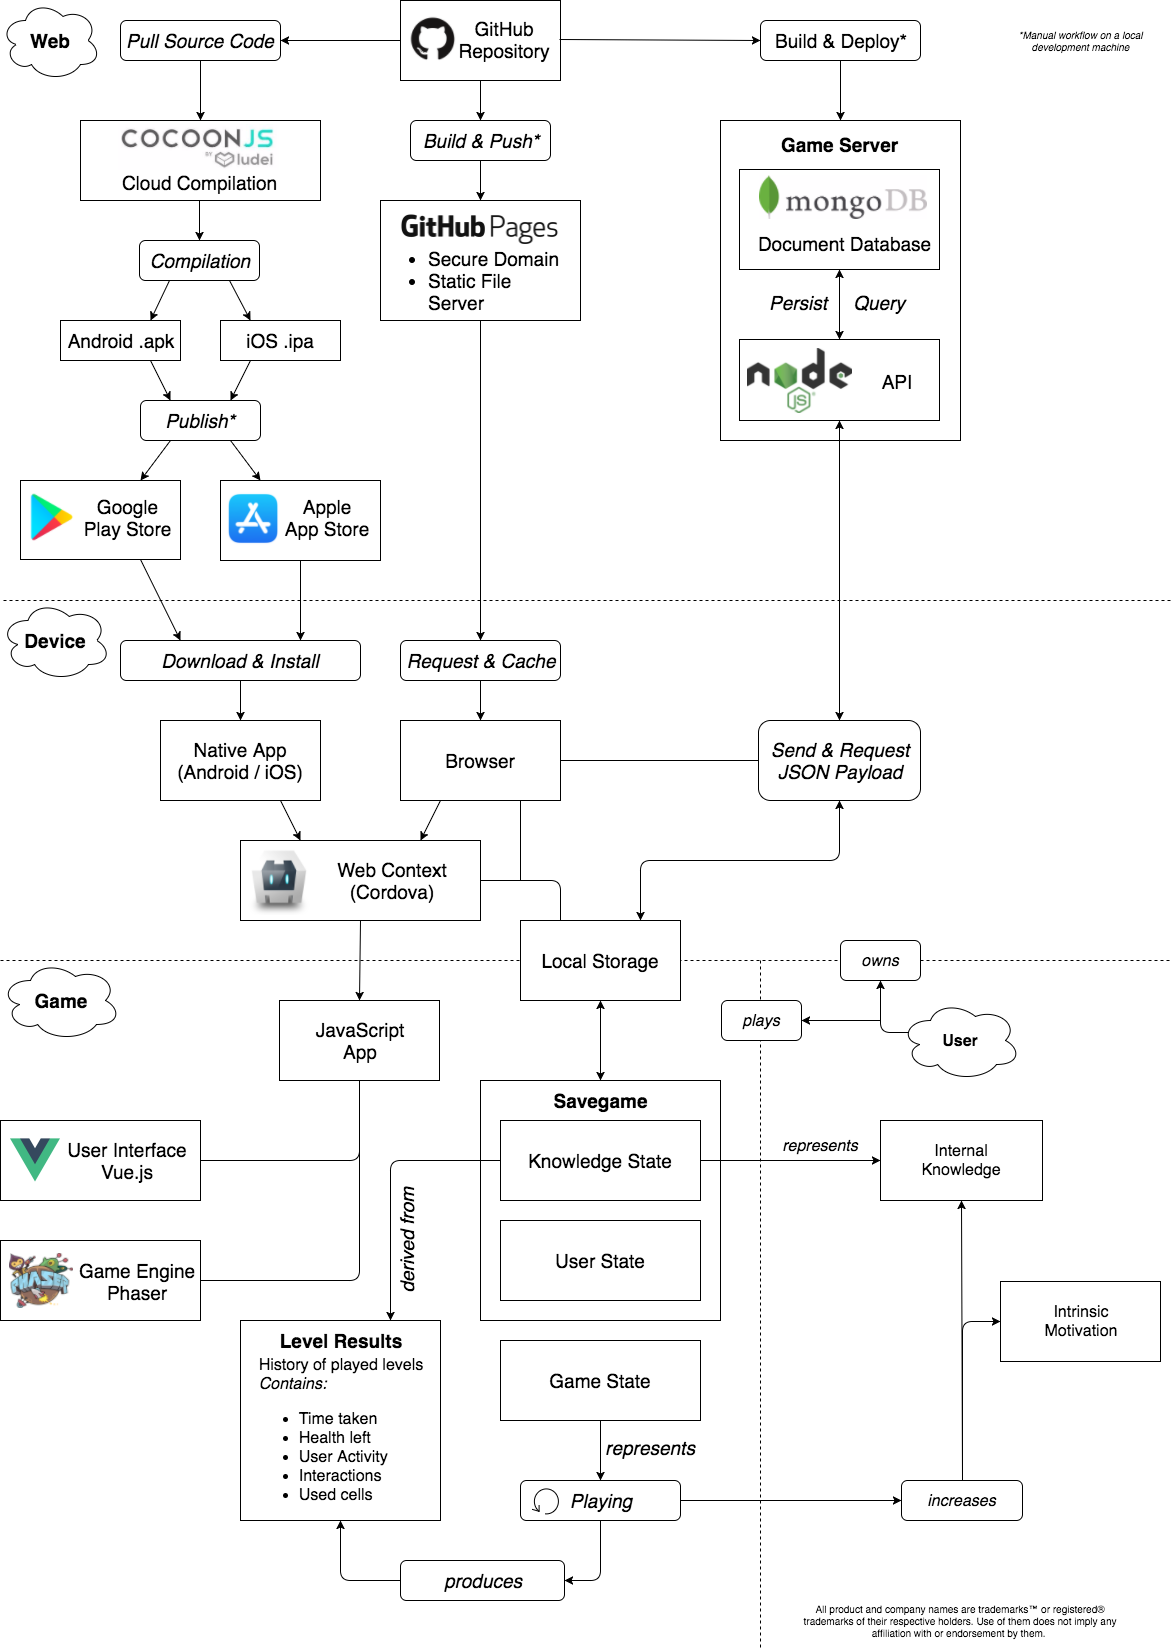
\includegraphics[width=15cm,keepaspectratio]{assets/architecture.png}
  \caption{System architecture overview}
  \label{fig_system_architecture}
\end{figure*}

\clearpage
% End: Full page System Description architecture
% End: SYSTEM DESCRIPTION

% Begin: DISCUSSION %
\section{Discussion} \label{discussion}
While developing this intelligent serious game a few issues were encountered and required further attention. Not all of these problems could be solved within the given time constraints and are therefore part of future research and work (See section \ref{future-work}).

Potential conflicts could surface with teachers and parents because the current design does not account for their role within the system. They might not believe in the effectiveness of the game's approach to learning and take a critical stance against usage in school or at home. There should be additional roles for teachers and parents which allow them access special views. These views could provide analytics about the activities and engagement of students. Teachers would benefit from insights into which topics their classes struggle with to incorporate that information into their lectures. However, there are not only data privacy issues with measuring activity. Further research and more importantly interviews with teachers, parents and schools are necessary to learn about their needs and requirements (See section \ref{future-work}).

Although the usage of smartphones is quite common today the assumption that every high school student owns a smartphone is wrong \cite{Lenhart2015TeensTeens}. Students without access to mobile devices would be unable to benefit from this game. This situation is remedied by the decision to build on web technologies. The game is available on the web and can be executed by all recent browsers. Even though, it was created with a mobile first approach it adopts to all screen sizes using responsive design. The only hard requirement left is access to a computer with a browser. Usually schools provide computer class rooms or family households have at least one shared computer available.

Being a mobile application it is possible for students to play the game in virtually any situation at any point in time. Naturally, there are scenarios, outlined in earlier sections (\ref{requirements} and \ref{startup}), where usage is non-ideal and potentially harmful towards the goal of supporting learning. The system deploys information alerts when it detects such a situation. They can be easily dismissed or even disabled in order to avoid dictating certain behaviour changes too much. It is possible that more sophisticated mechanisms are required to deal with this problem. Studying the usage of the game in the long run would be helpful to research this matter.

The approximation of the user's knowledge is a central problem of this research. Without a representation of this knowledge the game would present topics either too rarely or too often. The system uses the  \textit{Knowledge State} (Section \ref{knowledge-state}) as a learner model to approach this problem. It is derived from all \textit{Level Results} to keep track of the user's progress throughout the topics. In addition to that, using this detailed history of played levels helps to counteract a potential multi-user problem. If a student faces an ongoing challenge with a topic and asks a friend to solve the level a primitive system would assume that this topic is dealt with. Making use of the actual level history leads to further inclusion of the topic because of previous failed attempts.

Initial feedback on the game was gathered by conducting short term adoptive ethnographic studies and presenting the project in a poster session. One of the two short term studies was self-executed within the project's group members by using the game prototype multiple times throughout the day during the course of a week. The second study was carried out at the \enquote{Geert Groote College Amsterdam}\footnote{\url{http://ggca.nl/}, Accessed: 25-10-2017} with four secondary school students. Both studies showed early signs that most participants are inclined to skip text-based introductions. This theory further manifested itself during the poster session held in Science Park at University of Amsterdam. Visitors were able to play the tutorial of the prototype. In multiple cases feedback suggested the use of alternative approaches for introducing content. Especially providing an audio narrative for the tutorial was a reoccurring advice.

Lastly, during the initial stage of the project a more ambitious vision was set as a target in regards to the game itself. It included multiplayer aspects to create a more social setting and foster competitiveness, thereby increasing engagement. An essential part of multiplayer would be a game mode which pits two players against each other. One taking control of the human immune system and the other taking the opposing role of infections and diseases. Both players would need to know about the strength and weaknesses of all cells involved in order to succeed against each other. Due to the complexity and it being outside of the scope of this project this feature was pushed to future work (See section \ref{future-work}).
% End: DISCUSSION %

% Begin: CONCLUSION & FUTURE WORK %
\section{Conclusion \& Future Work} \label{future-work}
\enquote{Wreck Sam} is an intelligent serious game designed to educate in the field of Biology about the human immune system. It is intended to be used by high school students as a complementary learning tool in combination with traditional learning techniques. The visual and interactive approach of the game allows users to approach abstract concepts from a different angle. This helps to sustain motivation in students who would otherwise struggle to keep up and be frustrated instead. Moreover, it can increase intrinsic motivation by deeply engaging students within the topic through playing the game. The intelligent core system is responsible for modelling the user's knowledge progress and thereby dynamically selecting relevant topics to be used in levels.

% Begin: FUTURE WORK %
This paper and its accompanying prototype lay the groundwork for building an intelligent game which supports high school students learning about the immune system. However, more work is required to reach a production-ready stage which meets the needs of students.

First and foremost, an ethnographic study with actual high school students should be conducted. This vital step will reveal a lot of valuable insights about current learning environments in school and the problems students face while preparing their study material. It is important to use this feedback to further iterate on the proposed design to accommodate for usage scenarios which students could describe. Furthermore, observing students using the prototype can highlight design flaws or inconveniences in user experience.
This study could be extended to interview teachers and parents and find out about their needs and wishes for such an application. Including these groups into the research helps to understand how it could be useful for their goals in a classroom or while students study at home.

As a mean to limit the scope of the project it was only designed for teaching about the human immune system. It should be possible to extract the core intelligent system and adapt it for other topics. Research is necessary to evaluate whether the functionality can be applied to all school topics or if there are potential discrepancies.

Finally, the game itself is in a very early stage. Attention should be payed towards polishing cell sprites and their animations, working towards higher fidelity. They should match common representations in Biology books and mimic how interactions between real cells would look like. Multiplayer is an additional area which needs to be implemented. Nevertheless, this effort should be backed by prior research showing that multiplayer aspects would be beneficial towards the main goals (Section \ref{requirements}). However, judging from feedback received during initial prototype testing a sensible improvement would be providing audio voice-overs for the tutorial. The current prototype is only available as a mobile-first web version because of the inherent showcasing simplicity. For further elaborated testing it should be packaged as a native app and published to corresponding app stores. This increases immersion and usability by removing the browser's address bar, eases accessibility by providing an icon on the homescreen and lowers data usage by installing it to the device.
% End: FUTURE WORK %

% Begin: APPENDIX %
\section*{Appendix}

\subsection*{Appendix A: Inspiration}
The inspiration for this project stems from a video about the human immune system made by \enquote{Kurzgesagt - In a Nutshell} which was published on 1st of July in 2014. It is available on \textit{YouTube}:

\url{https://youtu.be/zQGOcOUBi6s}\footnote{Accessed: 14-09-2017}

\subsection*{Appendix B: GitHub Repository} \label{appendix-b}
The source code for this game is available on \textit{GitHub} at:

\url{https://github.com/marc1404/WreckSam}\footnote{Accessed: 13-10-2017}

\subsection*{Appendix C: Prototype} \label{prototype}
The prototype is hosted via \textit{GitHub Pages} at:

\url{https://marc1404.github.io/WreckSam/}\footnote{Accessed: 13-10-2017}

\subsection*{Appendix D: Poster}
On 18th of October 2017 the project was presented in form of a poster session at Science Park in Amsterdam. The poster is digitally available as a PDF-file inside the GitHub Repository:

\url{https://github.com/marc1404/WreckSam/blob/master/assets/documents/poster.pdf}\footnote{Accessed: 23-10-2017}
% End: APPENDIX %
